\subsection{Semantic Smart Contracts for Blockchain-based Services in the Internet of Things}
\label{subsec:semantic-smart-contract-iot}

Penelitian yang dilakukan oleh \cite{baqa2019semantic}, mengusulkan sebuah solusi untuk menemukan dan menggunakan Smart Contract untuk kegunaan spesifik, yang sulit dilakukan karena Smart Contract biasanya sudah dikompilasi dalam bentuk \textit{byte-code}, tanpa metadata yang terasosiasi. Solusi yang diusulkan adalah Semantic Smart Contract yang mengintegrasikan RESTful Semantic Web Technologies dalam Smart Contract, yang di-\textit{deploy} pada Blockchain Ethereum untuk melakukan \textit{indexing}, \textit{browsing}, dan melakukan anotasi terhadap sebuah Smart Contract. Penelitian ini menggunakan penelitian \cite{third2017linked} terkait Linked Data Indexing untuk meningkatkan \textit{discoverability}.

\begin{figure}
  \centering
  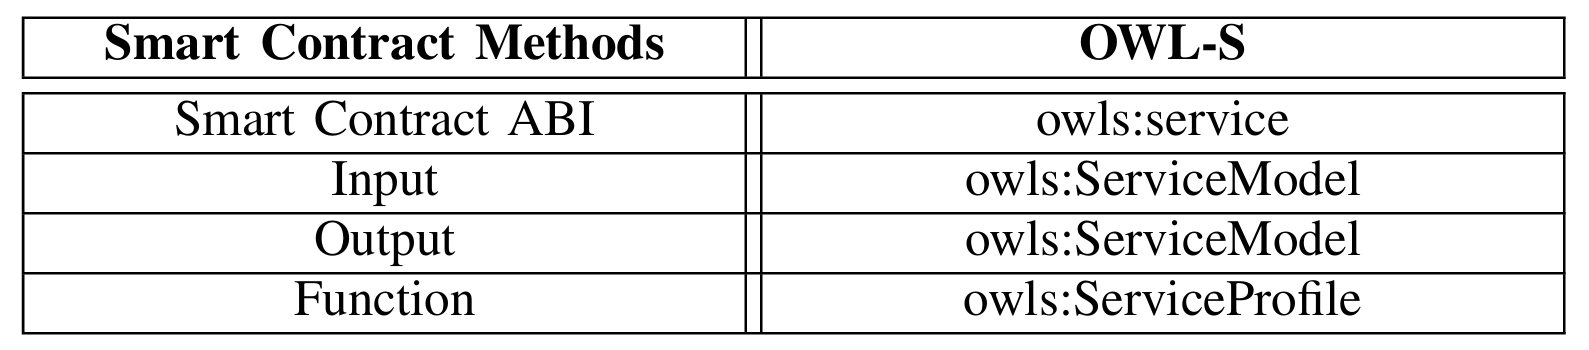
\includegraphics[width=0.7\textwidth]{resources/chapter-2/ssc-ontology-extension.png}
  \caption{Ekstensi OWL-S \parencite{baqa2019semantic}}
  \label{image:ekstensi-owl-s}
\end{figure}

Dalam pengembangan solusi yang diusulkan dalam penelitian ini, dilakukan ekstensi pada OWL-S Service Ontology, seperti pada gambar \ref{image:ekstensi-owl-s} dengan menginkorporasikan beberapa terminologi yang \textit{domain specific} seperti yang ada di dalam EthOn. Sehingga, Semantic Smart Contract dapat digunakan untuk memperkaya query untuk sebuah terminologi yang \textit{domain specific} antar beberapa \textit{distributed ledgers}, yang meningkatkan \textit{discoverability} dari sebuah aplikasi IoT yang terdesentralisasi.